\documentclass[varwidth=6.2in,border=3pt]{standalone}
\usepackage{tikz}
\usetikzlibrary{arrows.meta,decorations.pathreplacing,positioning,calc,fit}
\usepackage{amsmath}
\usepackage{algpseudocode}
\usepackage{newtxtext,newtxmath}
\newcommand{\code}[1]{\texttt{#1}}
\newcommand{\truesum}{\code{truesum}}
\begin{document}
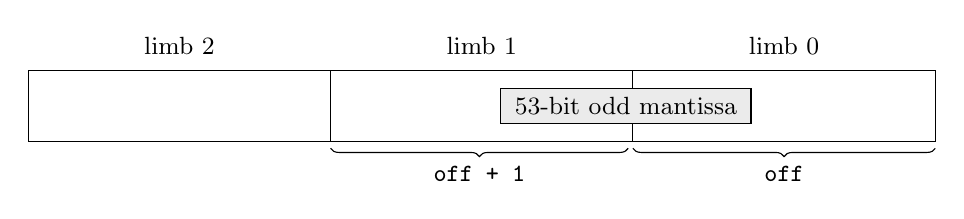
\begin{tikzpicture}[x=0.06cm,y=0.9cm,font=\small]
  \foreach \k in {2,1,0} { \pgfmathsetmacro{\x}{(2-\k)*64} \draw (\x,0) rectangle (\x+64,1); \node at (\x+32,1.35) {limb \k}; }
  \draw[fill=black!8] (100,0.25) rectangle (153,0.75);
  \node at (126.5,0.5) {53-bit odd mantissa};
  \draw[decorate,decoration={brace,mirror,amplitude=3pt}] (128,-0.1) -- (192,-0.1) node[midway,below=3pt] {\code{off}};
  \draw[decorate,decoration={brace,mirror,amplitude=3pt}] (64,-0.1) -- (127,-0.1) node[midway,below=3pt] {\code{off + 1}};
\end{tikzpicture}
\end{document}
